\documentclass[preprint]{sigplanconf}


\usepackage[utf8]{inputenc}
\usepackage{etex}
\usepackage{stmaryrd}
\usepackage{amsmath}
\usepackage{amsfonts}
\usepackage{amssymb}
\usepackage{mathtools}
\usepackage[amsmath,thmmarks]{ntheorem}
%\usepackage{algorithm2e}
\usepackage{tikz}
\usepackage{wrapfig}
\usepackage[numbers]{natbib}
\usepackage{mathpazo}
\usepackage{microtype}
\usepackage{booktabs}
\usepackage{mathpartir}
\newcommand\pfun{\mathrel{\ooalign{\hfil$\mapstochar\mkern5mu$\hfil\cr$\to$\cr}}}

\usepackage{hyperref}

\usetikzlibrary{shapes.geometric}
\usetikzlibrary{calc}
\usetikzlibrary{shapes.multipart}
\usetikzlibrary{arrows}

\urlstyle{sf}
\makeatletter
% Inspired by http://anti.teamidiot.de/nei/2009/09/latex_url_slash_spacingkerning/
% but slightly less kern and shorter underscore
\let\UrlSpecialsOld\UrlSpecials
\def\UrlSpecials{\UrlSpecialsOld\do\/{\Url@slash}\do\_{\Url@underscore}}%
\def\Url@slash{\@ifnextchar/{\kern-.11em\mathchar47\kern-.2em}%
   {\kern-.0em\mathchar47\kern-.08em\penalty\UrlBigBreakPenalty}}
\def\Url@underscore{\nfss@text{\leavevmode \kern.06em\vbox{\hrule\@width.3em}}}
\makeatother

\theorembodyfont{}
\newtheorem{theorem}{Theorem}
\newtheorem{lemma}[theorem]{Lemma}
\theoremstyle{nonumberplain}
\theoremheaderfont{\scshape}
\theoremsymbol{\ensuremath{\blacksquare}}
\theoremseparator{.}
\newtheorem{proof}{Proof}

\usepackage{listings}
\newcommand{\li}{\lstinline[style=Haskell]}
\lstnewenvironment{haskell}{\lstset{style=Haskell}}{}
\lstdefinestyle{Haskell}{language=Haskell
        ,columns=flexible
	,basewidth={.365em}
	,keepspaces=True
        ,texcl=true
%        ,escapechar=!
        ,basicstyle=\sffamily
        ,stringstyle=\itshape
        ,showstringspaces=false
        ,literate={->}{$\,\to\,$}2
                  {<-}{$\,\leftarrow\,$}2
                  {=>}{$\,\Rightarrow\,$}2
                  {→}{$\,\to\,$}2
%                  {\\}{\textlambda}1
                  {>>}{{>>}\hspace{-1pt}}2
%                  {+}{{$+$}}1
                  {[]}{[\,]\ }1
%                  {--}{{---\ }}1
                  {++}{{$+\!\!+$\ }}1
%                 {\ .}{{$\,\circ\,$}}2
                  {\ .\ }{{$\,\circ\,$}}2
	,keywords={type,data,where,let,in,case,of}
        }

\newcommand{\ci}{\lstinline[style=Cmm]}
\lstnewenvironment{cmm}{\lstset{style=Cmm}}{}
\lstdefinestyle{Cmm}{language=C
        ,columns=fullflexible
        ,texcl=true
%        ,escapechar=!
	,commentstyle=\sffamily\itshape
        ,basicstyle=\small\ttfamily
%        ,stringstyle=\itshape
%        ,showstringspaces=false
%	,keywords={type,data,where,let,in,case,of}
        }



\conferenceinfo{Haskell Symposium}{Sep 13 2012, Copenhagen} 
\copyrightyear{2012} 
\copyrightdata{Joachim Breitner}

\titlebanner{---Work in Progress---}
\preprintfooter{Joachim Breitner: dup -- Explicit un-sharing in Haskell}
\title{dup -- Explicit un-sharing in Haskell}
%\subtitle

\authorinfo{Joachim Breitner}{Karlsruhe Institute of Technology}{breitner@kit.edu}


\begin{document}
\maketitle
% \allowdisplaybreaks[1]

\begin{abstract}
We propose two operations to prevent sharing in Haskell that do not require modifying the data generating code, demonstrate their use and usefulness, and compare them to other approaches to preventing sharing. Our claims are supported by a formal semantics and a prototype implementation.
\end{abstract}

%\tableofcontents

\category{D.1.1}{Programming Techniques}{Applicative (Functional) Programming}
\category{D.3.3}{Programming Languages}{Language Constructs and Features}[Data types and structures]
\category{E.2}{Data storage representation}{}

\keywords Space leak, lazy evaluation, sharing, functional programming, natural semantics


\section{Introduction}

Due to the immutable nature of data in a pure functional programming language such as Haskell, there are many possibilities for sharing, i.e.\ one object in memory is used in multiple places in the program. In general, this is a good thing, as it can save both execution time (by not calculating the data again) and memory space (by not copying the data).

But there are cases where sharing can hurt, and sometimes hurt badly. A famous example is the following function:
\begin{haskell}
let f :: [Int] -> Int
    f xs = last xs + head xs
    l = [1..100000000]
in  f l
\end{haskell}
This program is space-leaky and will quickly run out of memory. If we substitute the term for \li-xs- in the body of \li-f- and evaluating that expression, it runs quickly and in constant memory. We have avoided the sharing of \li-xs- between the calls to \li-last- and \li-head- and the list elements can be garbage collected as soon as they have been consumed by \li-last-.

But this source transformation, as well as other source transformations to avoid sharing (see Section \ref{sec:unit} and \ref{sec:church}) is not always possible or desirable, e.g.\  when the parameter passed to \li-f- comes from library code not under the control of the programmer. For this case, we propose a new primitive operation \li-dup- which copies a (possibly unevaluated) value on the heap.
\pagebreak[3]
\begin{haskell}
data Box a = Box a
dup :: a -> Box a
\end{haskell}
Its value semantics are that of \li!(\x -> Box x)!; the wrapping in \li-Box- just serves the purpose of controlling the exact point of execution of \li-dup- by case-analyzing the \li-Box-. Using \li-dup- allows us to modify in the above example only the code of \li-f- to prevent sharing and achieve constant memory usage:
\begin{haskell}
let f xs = case dup xs of
    	Box xs' -> last xs' + head xs
    l = [1..100000000]
in  f l
\end{haskell}
In Section \ref{sec:unsharing} we demonstrate the use of \li-dup- and the other approaches on the more elaborate example introduced in Section \ref{sec:example}, taking on the programmer’s point of view.

An sharp-witted reader with knowledge of a typical implementation of a Haskell runtime might already have noticed that just copying the object on the heap representing the parameter \li-xs- might not be enough: If, for example, the first cons-cell of \li-xs- is already evaluated, then \li-dup xs- will copy that cell, but the thunk representing the tail of the list will still be shared between \li-xs'- and \li-xs-, and \li-f- will again devour memory. Such things may occur without the programmer’s knowledge, e.g.\ during a compiler optimization pass.

To that end, we propose a variant of \li-dup-, called \li-deepDup-, which not only copies its parameter, but also replaces every reference to other objects in the parameter by calls to \li-deepDup-. These calls are, as one would expect for anything related to Haskell, lazy and only copy the referenced object if and when it is needed. In other words: After evaluating a function which only works on a \li-deepDup-’ed copy of its parameters, nothing this evaluation created on the heap is referenced anymore, unless it is referenced by the function's return value (this is formalized in Theorem \ref{thm:deepdup}).

Our specific contributions are:
\begin{itemize}
\item We introduce primitives that give the programmer the possibility to explicitly prevent sharing.
\item In contrast approaches based on source transformations, using \li-dup- and \li-deepDup- does \emph{not} require changes to the generating code.
\item We provide precise semantics in the context of Launchbury’s natural semantics for Lazy Evaluation (Section \ref{sec:semantics}) and prove that the recursive variant \li-deepDup- is effective.
\item We show the feasibility of our approach using a proof-of-concept implementation targeting code compiled by an unmodified GHC. (Section \ref{sec:prototype})
\end{itemize}

\pagebreak[3]
\section{The running example}
\label{sec:example}

For the remainder of the paper, we will use one running example to demonstrate and discuss the use of \li-dup-. The task at hand is to find a path through a (possibly infinite) tree that maximizes some valuation of the nodes. So abstractly, we have a type \li-S- of states, a valuation function \li-value-, an initial state \li-init- and for every state \li-s-, a list of successor states \li-succs s- (see also Figure \ref{fig:ex}).

\begin{figure}
\begin{haskell}
-- The problem specification
type S = ...
init :: S
succs :: S -> [S]
value :: S -> Integer

-- The search tree code
data Tree = Node S [Tree]
tree :: S -> Tree
tree s = Node s (map tree (succs s))
depth :: Int
solve :: Tree -> [S]
solve (Node n ts) = n : solve picked
  where
  rated = [ (t, rate depth t) | t <- ts ]
  picked = fst (maximumBy (comparing snd) rated)
rate :: Tree -> Integer
rate 0 (Node s _) = value s
rate d (Node _ ts) = maximum (map (rate (d-1)) ts)

main = do
  let t = tree init
  print $ solve t !! 10000
  doSomethingElseWith t
\end{haskell}
\caption{The running example}
\label{fig:ex}
\end{figure}

Based on these functions, we define a search tree and a solver. The solver picks the successor with the highest rating, whereas the rating is the highest value of nodes at a configurable depth.

Assume a constant number of successors $b$ and that the value of \li-depth- is $d$. Consider what happens when the \li-main- function in Figure \ref{fig:ex} is run: To figure out the first 10\,000 elements of the solution, the \li-rate- function will evaluate lots of nodes that will \emph{not} be picked for the solution. But as they are still referenced by the tree \li-t-, the garbage collector cannot get rid of them. So in addition to the  10\,000 interesting nodes, roughly $10\,000\cdot (b-1)\cdot b^{d-1}$ nodes are evaluated that the programmer knows are not required to be kept around. The first row of Figure \ref{fig:evaluation} depicts the heap during this evaluation, with $d=1$ and $b=2$.

\newcommand{\stats}[1]{\ref*{#1}}
More concretely with $d=4$, $b=4$, \li-type S = Word32- and a very cheap \li-succs- function, this program requires \stats{stats:Original:Shared:mem}~MB of system memory and runs in \stats{stats:Original:Shared:time} seconds.%
\footnote{All statistics are obtained on a machine with 2.5~GHz and 6~GB of RAM. The complete code used to generate these statistics is available in the \ci!ghc-dup! repository, \url{http://darcs.nomeata.de/ghc-dup}.} Sharing is indeed the problem here: If we remove the last line of \li-main-, the program runs in \stats{stats:Original:Unshared:mem}~MB of memory and takes \stats{stats:Original:Unshared:time} seconds.

\section{Unsharing the example}
\label{sec:unsharing}

\begin{figure*}
\centering
\makeatletter
\begin{tabular}{lrrrrrrrrrr}
 \\
& \multicolumn{2}{c}{no sharing}& \multicolumn{2}{c}{shared tree}& \multicolumn{2}{c}{add. thunk}& \multicolumn{2}{c}{partly eval'ed}& \multicolumn{2}{c}{fully eval'ed} \\
& MB & sec.& MB & sec.& MB & sec.& MB & sec.& MB & sec. \\ \midrule 
original& {\def\@currentlabel{2}\label{stats:Original:Unshared:mem}2} & {\def\@currentlabel{3.72}\label{stats:Original:Unshared:time}3.72}& {\def\@currentlabel{4\,189}\label{stats:Original:Shared:mem}4\,189} & {\def\@currentlabel{14.07}\label{stats:Original:Shared:time}14.07}& {\def\@currentlabel{4\,188}\label{stats:Original:SharedThunk:mem}4\,188} & {\def\@currentlabel{14.02}\label{stats:Original:SharedThunk:time}14.02}& {\def\@currentlabel{4\,188}\label{stats:Original:SharedEvaled:mem}4\,188} & {\def\@currentlabel{13.99}\label{stats:Original:SharedEvaled:time}13.99}& {\def\@currentlabel{4\,189}\label{stats:Original:SharedFull:mem}4\,189} & {\def\@currentlabel{18.12}\label{stats:Original:SharedFull:time}18.12} \\
\textsf{solveDup}& {\def\@currentlabel{2}\label{stats:SolveDup:Unshared:mem}2} & {\def\@currentlabel{3.71}\label{stats:SolveDup:Unshared:time}3.71}& {\def\@currentlabel{2}\label{stats:SolveDup:Shared:mem}2} & {\def\@currentlabel{3.80}\label{stats:SolveDup:Shared:time}3.80}& {\def\@currentlabel{4\,188}\label{stats:SolveDup:SharedThunk:mem}4\,188} & {\def\@currentlabel{14.29}\label{stats:SolveDup:SharedThunk:time}14.29}& {\def\@currentlabel{4\,188}\label{stats:SolveDup:SharedEvaled:mem}4\,188} & {\def\@currentlabel{14.26}\label{stats:SolveDup:SharedEvaled:time}14.26}& {\def\@currentlabel{4\,188}\label{stats:SolveDup:SharedFull:mem}4\,188} & {\def\@currentlabel{18.30}\label{stats:SolveDup:SharedFull:time}18.30} \\
\textsf{rateDup}& {\def\@currentlabel{2}\label{stats:RateDup:Unshared:mem}2} & {\def\@currentlabel{1.57}\label{stats:RateDup:Unshared:time}1.57}& {\def\@currentlabel{5}\label{stats:RateDup:Shared:mem}5} & {\def\@currentlabel{1.58}\label{stats:RateDup:Shared:time}1.58}& {\def\@currentlabel{5}\label{stats:RateDup:SharedThunk:mem}5} & {\def\@currentlabel{1.58}\label{stats:RateDup:SharedThunk:time}1.58}& {\def\@currentlabel{5}\label{stats:RateDup:SharedEvaled:mem}5} & {\def\@currentlabel{1.57}\label{stats:RateDup:SharedEvaled:time}1.57}& {\def\@currentlabel{4\,189}\label{stats:RateDup:SharedFull:mem}4\,189} & {\def\@currentlabel{18.46}\label{stats:RateDup:SharedFull:time}18.46} \\
\textsf{solveDeepDup}& {\def\@currentlabel{2}\label{stats:SolveDeepDup:Unshared:mem}2} & {\def\@currentlabel{3.74}\label{stats:SolveDeepDup:Unshared:time}3.74}& {\def\@currentlabel{2}\label{stats:SolveDeepDup:Shared:mem}2} & {\def\@currentlabel{3.77}\label{stats:SolveDeepDup:Shared:time}3.77}& {\def\@currentlabel{2}\label{stats:SolveDeepDup:SharedThunk:mem}2} & {\def\@currentlabel{3.68}\label{stats:SolveDeepDup:SharedThunk:time}3.68}& {\def\@currentlabel{2}\label{stats:SolveDeepDup:SharedEvaled:mem}2} & {\def\@currentlabel{3.68}\label{stats:SolveDeepDup:SharedEvaled:time}3.68}& {\def\@currentlabel{4\,188}\label{stats:SolveDeepDup:SharedFull:mem}4\,188} & {\def\@currentlabel{18.12}\label{stats:SolveDeepDup:SharedFull:time}18.12} \\
unit lifting& {\def\@currentlabel{1}\label{stats:Unit:Unshared:mem}1} & {\def\@currentlabel{1.12}\label{stats:Unit:Unshared:time}1.12}& {\def\@currentlabel{1}\label{stats:Unit:Shared:mem}1} & {\def\@currentlabel{1.12}\label{stats:Unit:Shared:time}1.12}& {\def\@currentlabel{1}\label{stats:Unit:SharedThunk:mem}1} & {\def\@currentlabel{1.12}\label{stats:Unit:SharedThunk:time}1.12}& {\def\@currentlabel{1}\label{stats:Unit:SharedEvaled:mem}1} & {\def\@currentlabel{1.13}\label{stats:Unit:SharedEvaled:time}1.13}& {\def\@currentlabel{2}\label{stats:Unit:SharedFull:mem}2} & {\def\@currentlabel{2.26}\label{stats:Unit:SharedFull:time}2.26} \\
church encoding& {\def\@currentlabel{2}\label{stats:Church:Unshared:mem}2} & {\def\@currentlabel{5.97}\label{stats:Church:Unshared:time}5.97}& {\def\@currentlabel{2}\label{stats:Church:Shared:mem}2} & {\def\@currentlabel{5.96}\label{stats:Church:Shared:time}5.96}& {\def\@currentlabel{2}\label{stats:Church:SharedThunk:mem}2} & {\def\@currentlabel{5.97}\label{stats:Church:SharedThunk:time}5.97}& {\def\@currentlabel{2}\label{stats:Church:SharedEvaled:mem}2} & {\def\@currentlabel{6.00}\label{stats:Church:SharedEvaled:time}6.00}& {\def\@currentlabel{2}\label{stats:Church:SharedFull:mem}2} & {\def\@currentlabel{11.86}\label{stats:Church:SharedFull:time}11.86} \\
\end{tabular}
\makeatother

\caption{Time and space performance}
\label{fig:stats}
\end{figure*}

\begin{figure*}
\centering
{
\sffamily
\begin{tikzpicture}
[level/.style={sibling distance=20mm/2^#1,level distance=6mm},
every node/.style={inner sep=1pt},
solve/.style={draw,circle,inner sep=1pt},
rate/.style={draw,rectangle,inner sep=2pt},
%every path/.style={->},
]
\matrix[column sep={5mm},row sep=4mm] (matrix) {
\node[left]{\rmfamily original:};
&
\node[solve] (root) {T};
\draw (root.north) -- +(0mm,2mm);
&

&

\node[solve] (root) {N}
child {node [rate] {T}}
child {node  {T}};
\draw (root.north) -- +(0mm,2mm);

&
\node[solve] (root) {N}
child {node [rate] {N}
	child {node  {N} child {node {T}} child {node {T}}}
	child {node  {N} child {node {T}} child {node {T}}}
	}
child {node  {T}};
\draw (root.north) -- +(0mm,2mm);

&
\node[solve] (root) {N}
child {node  {N}
	child {node  {N} child {node {T}} child {node {T}}}
	child {node  {N} child {node {T}} child {node {T}}}
	}
child {node[rate]  {N}
	child {node  {N} child {node {T}} child {node {T}}}
	child {node  {N} child {node {T}} child {node {T}}}
	}
;
\draw (root.north) -- +(0mm,2mm);

&

\node (root) {N}
child {node  {N}
	child {node  {N} child {node {T}} child {node {T}}}
	child {node  {N} child {node {T}} child {node {T}}}
	}
child {node [solve] {N}
	child {node  {N} child {node {T}} child {node {T}}}
	child {node  {N} child {node {T}} child {node {T}}}
	};
\draw (root.north) -- +(0mm,2mm);

\\
\node[left]{\rmfamily \textsf{solveDup}:};
&
\node[solve] (root) {T};
\draw (root.north) -- +(0mm,2mm);
&

\node  at (-6mm,0mm) (root) {T};
\draw (root.north) -- +(0mm,2mm);
\node[solve] (root2) {T};
\draw[double] (root) -- (root2);
&

\node  at (-6mm,0mm) (root) {T};
\draw (root.north) -- +(0,2mm);
\node[solve](root2) {N}
child {node [rate] {T}}
child {node  {T}};
\draw[double] (root) -- (root2);

&
\node at (-6mm,0mm)  (root) {T};
\draw (root.north) -- +(0,2mm);
\node[solve](root2) {N}
child {node [rate] {N}
	child {node  {N} child {node {T}} child {node {T}}}
	child {node  {N} child {node {T}} child {node {T}}}
	}
child {node  {T}};
\draw (root.north) -- +(0,2mm);
\draw[double] (root) -- (root2);

&
\node at (-6mm,0mm)  (root) {T};
\draw (root.north) -- +(0,2mm);
\node[solve](root2) {N}
child {node {N}
	child {node  {N} child {node {T}} child {node {T}}}
	child {node  {N} child {node {T}} child {node {T}}}
	}
child {node [rate] {N}
	child {node  {N} child {node {T}} child {node {T}}}
	child {node  {N} child {node {T}} child {node {T}}}
	}
;
\draw (root.north) -- +(0,2mm);
\draw[double] (root) -- (root2);

&

\node  at (-6mm,0mm) (root) {T};
\draw (root.north) -- +(0,2mm);
\draw [gray] node(root2) {N}
child {node  {N}
	child {node  {N} child {node {T}} child {node {T}}}
	child {node  {N} child {node {T}} child {node {T}}}
	}
child {node[solve,black] {N}
	child[black] {node  {N} child {node {T}} child {node {T}}}
	child[black] {node  {N} child {node {T}} child {node {T}}}
	};
\draw (root.north) -- +(0,2mm);
\draw[gray,double] (root) -- (root2);

\\
\node[left]{\rmfamily \textsf{rateDup}:};
&
\node[solve] (root) {T};
\draw (root.north) -- +(0mm,2mm);
&

\node[solve] (root) {N}
child {node [rate] {T}}
child {node  {T}};
\draw (root.north) -- +(0mm,2mm);

&
\node[solve] (root) {N}
child {node (rate) {T}}
child {node  {T}};
\path (rate) +(6mm,0) node[rate] (rate2) {T};
\draw (root.north) -- +(0mm,2mm);
\draw[double] (rate) -- (rate2);


&
\node[solve] (root) {N}
child {node (rate) {T}
 +(6mm,0) node[rate] (rate2) {N}
	child {node  {N} child {node {T}} child {node {T}}}
	child {node  {N} child {node {T}} child {node {T}}}
	}
child {node  {T}};
\draw (root.north) -- +(0mm,2mm);
\draw[double] (rate) -- (rate2);

&
\node[solve] (root) {N}
child {node (rate') {T}
 +(6mm,0) node[gray] (rate'2) {N}
	child[gray] {node  {N} child {node {T}} child {node {T}}}
	child[gray] {node  {N} child {node {T}} child {node {T}}}
	}
child {node (rate) {T}
 +(6mm,0) node[rate] (rate2) {N}
	child {node  {N} child {node {T}} child {node {T}}}
	child {node  {N} child {node {T}} child {node {T}}}
	}
;
\draw (root.north) -- +(0mm,2mm);
\draw[double] (rate) -- (rate2);
\draw[double,gray] (rate') -- (rate'2);

&

\node (root) {N}
child {node (t1) {T}
 +(6mm,0) node[gray] (t1') {N}
	child[gray] {node  {N} child {node {T}} child {node {T}}}
	child[gray] {node  {N} child {node {T}} child {node {T}}}
	}
child {node [solve] (t2) {T}
 +(6mm,0) node[gray] (t2') {N}
	child[gray] {node  {N} child {node {T}} child {node {T}}}
	child[gray] {node  {N} child {node {T}} child {node {T}}}
	};
\draw (root.north) -- +(0mm,2mm);
\draw[gray,double] (t1) -- (t1');
\draw[gray,double] (t2) -- (t2');
\\
}
;

\path (matrix.south west)
%+(0,10mm)
node [below right] {
\parbox{88mm}{
\rmfamily
%\textbf{Legend:}
%\\
\textsf{T}: thunk, \textsf{N}: node, $=$: dup’ed closure,
 \textcolor{gray}{garbage},
\\
\begin{tikzpicture}[baseline=(n.base)]
\node[solve] (n) {T};
\end{tikzpicture}:
 current argument of solve,
 %\\
\begin{tikzpicture}[baseline=(n.base)]
\node[rate] (n) {T};
\end{tikzpicture}:
 current argument of rate
}
};
\end{tikzpicture}
}
\caption{The heap during original and \textsf{dup}’ed evaluation}
\label{fig:evaluation}
\end{figure*}

We want to improve the space performance of the program in the example and thus, due to the saved work in the garbage collector, also the runtime performance. In the following, we use \li-dup-, first wrapping the argument of \li-solve-, then the argument of \li-rate-, and \li-deepDup-. We also try two variants that work without new primitives but require refactoring the generating code. The statistics are collected in Figure \ref{fig:stats}, where all six strategies are applied to an otherwise unreferenced tree first and then to a tree with a live reference, either unevaluated, wrapped in another thunk, partly evaluated or fully evaluated.


\subsection{Using dup}

We now modify the example to use our new primitives. There are a few choices in doing so, with different trade-offs. One candidate for \li-dup-ifying is the function \li-solve-: We know that the parameter \li-t- to \li-solve- is an unevaluated expression, and decoupling that from the \li-t- that we pass to \li-doSomethingElseWith- will allow the garbage collector to clean up the tree as \li-solve- proceeds to process it (Figure \ref{fig:evaluation}, second row). So we wrap \li-solve- in \li-solveDup- and use that in \li-main-.
\begin{haskell}
solveDup t = case dup t of Box t' -> solve t'
\end{haskell}
And indeed, we have almost achieved the performance of the original program without sharing: \stats{stats:SolveDup:Shared:mem}~MB and \stats{stats:SolveDup:Shared:time} seconds.


Another candidate for \li-dup-ifying is the function \li-rate-:
As this is the function whose return value is taken into account when deciding whether to pick the argument or not, we know that in most cases, its argument will not be used any more. Therefore, by creating a wrapper \li-rateDup- that duplicates the argument, and using that in \li-solve-, we allow for the argument and all its children to be garbage collected once \li-rate- has finished.
\begin{haskell}
rateDup t = case dup t of Box t' -> rate t'
\end{haskell}

Both the runtime and the memory footprint of the program are greatly reduced: It uses \stats{stats:RateDup:Shared:mem}~MB of memory and \stats{stats:RateDup:Shared:time} seconds to finish. It is surprising that this even surpasses the speed of the original program without sharing. The reason is that with \li-rate- wrapped in \li-dup-, the first child of the node under inspection of \li-solve- can be freed already when its next child is evaluated by \li-rate- (Figure \ref{fig:evaluation}, last row, second-to-last column), so even less work needs to be done by the copying garbage collector.

\subsection{Using deepDup}
\begin{figure*}
\centering
{
\sffamily
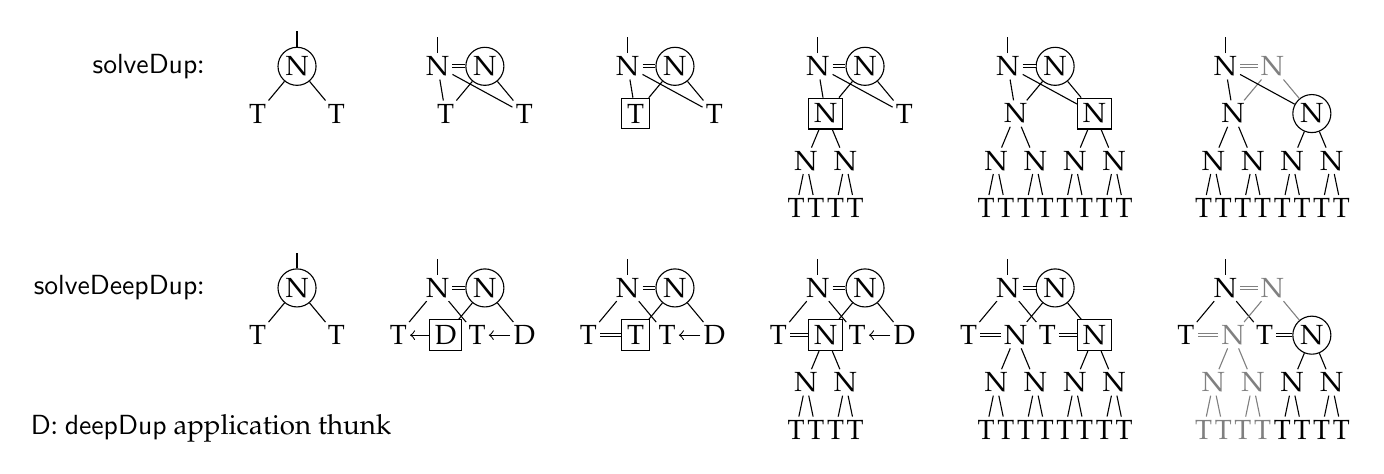
\begin{tikzpicture}
[level/.style={sibling distance=20mm/2^#1,level distance=6mm},
every node/.style={inner sep=1pt},
solve/.style={draw,circle,inner sep=1pt},
rate/.style={draw,rectangle,inner sep=2pt},
]
\matrix[column sep={5mm},row sep=4mm] (matrix) {
\node[left]{\rmfamily \textsf{solveDup}:};
&
\node[solve] (root) {N}
child {node  {T}}
child {node  {T}};
\draw (root.north) -- +(0mm,2mm);
&

\node  at (-6mm,0mm) (root) {N};
\draw (root.north) -- +(0mm,2mm);
\node[solve] (root2) {N}
child {node  {T}}
child {node  {T}};
\draw[double] (root) -- (root2);
\draw (root) -- (root2-1);
\draw (root) -- (root2-2);
&

\node  at (-6mm,0mm) (root) {N};
\draw (root.north) -- +(0,2mm);
\node[solve](root2) {N}
child {node [rate] {T}}
child {node  {T}};
\draw[double] (root) -- (root2);
\draw (root) -- (root2-1);
\draw (root) -- (root2-2);

&
\node at (-6mm,0mm)  (root) {N};
\draw (root.north) -- +(0,2mm);
\node[solve](root2) {N}
child {node [rate] {N}
	child {node  {N} child {node {T}} child {node {T}}}
	child {node  {N} child {node {T}} child {node {T}}}
	}
child {node  {T}};
\draw (root.north) -- +(0,2mm);
\draw[double] (root) -- (root2);
\draw (root) -- (root2-1);
\draw (root) -- (root2-2);

&

\node  at (-6mm,0mm) (root) {N};
\draw (root.north) -- +(0,2mm);
\draw  node[solve] (root2) {N}
child {node  {N}
	child {node  {N} child {node {T}} child {node {T}}}
	child {node  {N} child {node {T}} child {node {T}}}
	} 
child {node[rate] {N}
	child {node  {N} child {node {T}} child {node {T}}}
	child {node  {N} child {node {T}} child {node {T}}}
	};
\draw (root.north) -- +(0,2mm);
\draw[double] (root) -- (root2);
\draw (root) -- (root2-1);
\draw (root) -- (root2-2);

&

\node  at (-6mm,0mm) (root) {N};
\draw (root.north) -- +(0,2mm);
\draw  node[gray] (root2) {N}
child {node  {N}
	child[black] {node  {N} child {node {T}} child {node {T}}}
	child[black] {node  {N} child {node {T}} child {node {T}}}
	edge from parent[gray]
	} 
child {node[solve,black] {N}
	child[black] {node  {N} child {node {T}} child {node {T}}}
	child[black] {node  {N} child {node {T}} child {node {T}}}
	edge from parent[gray]
	};
\draw (root.north) -- +(0,2mm);
\draw[gray,double] (root) -- (root2);
\draw (root) -- (root2-1);
\draw (root) -- (root2-2);

\\
\node[left]{\rmfamily \textsf{solveDeepDup}:};
&
\node[solve] (root) {N}
child {node  {T}}
child {node  {T}};
\draw (root.north) -- +(0mm,2mm);
&

\node  at (-6mm,0mm) (root) {N}
child {node  {T}}
child {node  {T}}
;
\draw (root.north) -- +(0mm,2mm);
\node[solve] (root2) {N}
child {node[rate]  {D}}
child {node  {D}};
\draw[double] (root) -- (root2);
\draw[->] (root2-1) -- (root-1);
\draw[->] (root2-2) -- (root-2);

&

\node  at (-6mm,0mm) (root) {N}
child {node  {T}}
child {node  {T}}
;
\draw (root.north) -- +(0mm,2mm);
\node[solve] (root2) {N}
child {node[rate]  {T}}
child {node  {D}};
\draw[double] (root) -- (root2);
\draw[double] (root2-1) -- (root-1);
\draw[->] (root2-2) -- (root-2);

&

\node  at (-6mm,0mm) (root) {N}
child {node  {T}}
child {node  {T}}
;
\draw (root.north) -- +(0mm,2mm);
\node[solve] (root2) {N}
child {node[rate]  {N}
	child {node  {N} child {node {T}} child {node {T}}}
	child {node  {N} child {node {T}} child {node {T}}}
	}
child {node  {D}};
\draw[double] (root) -- (root2);
\draw[double] (root2-1) -- (root-1);
\draw[->] (root2-2) -- (root-2);

&
\node  at (-6mm,0mm) (root) {N}
child {node  {T}}
child {node  {T}}
;
\draw (root.north) -- +(0mm,2mm);
\node[solve] (root2) {N}
child {node  {N}
	child {node  {N} child {node {T}} child {node {T}}}
	child {node  {N} child {node {T}} child {node {T}}}
	}
child {node[rate]  {N}
	child {
		node  {N} child {node {T}} child {node {T}}
		}
	child {
		node  {N} child {node {T}} child {node {T}}
		}
	edge from parent
};
\draw[double] (root) -- (root2);
\draw[double] (root2-1) -- (root-1);
\draw[double] (root2-2) -- (root-2);


&
\node  at (-6mm,0mm) (root) {N}
child {node  {T}}
child {node  {T}}
;
\draw (root.north) -- +(0mm,2mm);
\node[gray] (root2) {N}
child[gray] {node  {N}
	child {node  {N} child {node {T}} child {node {T}}}
	child {node  {N} child {node {T}} child {node {T}}}
	}
child {node[solve]  {N}
	child[black] {
		node  {N} child {node {T}} child {node {T}}
		}
	child[black] {
		node  {N} child {node {T}} child {node {T}}
		}
	edge from parent[gray]
};
\draw[double,gray] (root) -- (root2);
\draw[double,gray] (root2-1) -- (root-1);
\draw[double] (root2-2) -- (root-2);

\\
}
;
\path (matrix.south west)
%+(0,10mm)
node [above right] {
\parbox{88mm}{
\rmfamily
%\textbf{Legend:}
%\\
\textsf{D}: \textsf{deepDup} application thunk
}
};
\end{tikzpicture}
}
\caption{Comparing \textsf{solveDup} and \textsf{solveDeepDup} applied to a partly evaluated tree}
\label{fig:deepevaluation}
\end{figure*}

\label{sec:deepdup}
Using \li-dup- is a fragile business and requires the programmer to have a very good idea about what is happening at runtime. The approach above is fragile and will fail, for example, in two common situations: If the argument to \li-solveDup- is not just the tree \li-t- but rather an expression that references \li-t-, e.g.\ \li-fstChild t- where \li!fstChild :: Tree -> Tree! does what its name indicates, then \li-dup- will only copy this unevaluated expression, but both copies will reference the same unevaluated expression for~\li-t-, and we are back at the original performance (\stats{stats:SolveDup:SharedThunk:mem}~MB, \stats{stats:SolveDup:SharedThunk:time} seconds).

The same effect occurs if the tree is already partly evaluated. This may even be caused by a compiler transformation, e.g.\ the wrapper/worker transformation, assuming that \li-doSomethingElseWith- is strict  in its argument \citep{unboxed}. Then, the parameter \li-t- is the \li-Node- constructor referencing other nodes or unevaluated trees, and copying the constructor does not help to prevent sharing the referenced data, as shown in the first row of Figure \ref{fig:deepevaluation}.

This is where \li-deepDup- comes in: It will not only copy the object specified by its parameter, but also change all references therein so that before they are evaluated, \li-deepDup- copies them. So we wrap \li-solve- in a call to \li-deepDup-:
\begin{haskell}
solveDeepDup t = case deepDup t of Box t' -> solve t'
\end{haskell}
Now we achieve the performance of a successful run with \li-dup- (\stats{stats:SolveDeepDup:SharedThunk:mem}~MB and \stats{stats:SolveDeepDup:SharedThunk:time} seconds), but also in the cases where \li-t- has already been partly evaluated or is wrapped in another unevaluated expression. The second row of Figure \ref{fig:deepevaluation} shows \li-deepDup- at work.

Using \li-deepDup- is therefore more reliable and easier to handle: The programmer need not have an exact idea of the evaluation state of the arguments when \li-deepDup- is called. And the recursive copying is surprisingly cheap: Even when the tree is already fully evaluated, e.g. by an earlier call to \li-solve t !! 10000-, the runtime stays the same within the precision of the benchmark.
%\footnote{In fact, it is reliably reduced by about one percent; the reason is not yet clear to us.}

%\section{Other approaches to unsharing}
%\label{sec:sourcetrans}

\subsection{The unit type argument pattern}

The problem at hand is, of course, not new, and Haskell programmers have solved it one way or the other before, by rewriting the code to allow more control over sharing.

\label{sec:unit}

A common approach is to replace values that you do not want to be shared by functions, e.g.\ by wrapping a bound expression \li-let x = e- into a lambda expression \li!let x = \() -> e!. At every point in the program where \li-e- is required, one can get the value of it using \li-x ()-; there will be no sharing between different calls to \li-x ()-

One needs to be careful, though, as some compiler optimization can introduce unwanted sharing again. The code
\begin{haskell}
xs :: () -> [Int]
xs () = [1..10000000]
main = do
    print (last (xs ()))
    print (head (xs ()))
\end{haskell}
works as expected without optimization. Passing  \ci!-O! to GHC results in sharing again, as a result of the full laziness transformation. In fact, in a discussion of this example on the GHC bug tracker \citep{spaceleakbug}, Claus Reinke suggests an operation like \li-dup- to solve this.
% http://hackage.haskell.org/trac/ghc/ticket/917

If, however, the type signature of \li-xs- is not given, then no unwanted sharing happens even with \ci!-O!. The inferred, most general type of \li-xs- is polymorphic with type class constraints. This implies that additional parameters are being passed under the hood and they successfully prevent sharing.

Applying this pattern to our problem, and aiming for a tree with unshareable subtrees, we can define the following types:
\begin{haskell}
data UTree' = UNode S [UTree]
type UTree = () -> UTree'
\end{haskell}
The required changes to the functions on trees are mechanical and guided by the type checker. The resulting code, when not hit by some optimization-induced re-sharing, shows very good time and space complexity. If sharing is desired at some points of the program, those parts will have to work with the regular \li-Tree- type, possibly leading to a duplication of code.

\subsection{Church encoding}
\label{sec:church}

An alternative is to restructure the program so that the value that must not be shared is not represented using data constructors but rather as a higher-order function \citep{churchenc,olegchurchenc}. This transformation is known as the Church encoding of a data type. For the tree in our running example we would obtain the following type and conversion functions:
\begin{haskell}
type CTree = forall a. (S -> [a] -> a) -> a
toCTree :: Tree -> CTree
toCTree (Node s ts) f = f s $ map (\t -> toCTree t f) ts
fromCTree :: CTree -> Tree
fromCTree ct = ct Node
\end{haskell}

A church-encoded tree corresponding to the value \li-tree s- can be nicely created with the following code:
\begin{haskell}
ctree :: S -> CTree
ctree s f = f s $ map (\s' -> ctree s' f) (succs s)
\end{haskell}

Unfortunately, adapting \li-solve- to this type is a non-trivial task, as the two recursions happening therein (\li-solve- and \li-rate-) need to be folded into one pass:
\begin{haskell}
csolve :: CTree -> [S]
csolve t = fst (t csolve')
  where
  csolve' :: S -> [([S],[Int])] -> ([S],[Int])
  csolve' n rc = 
    ( n : fst (maximumBy (comparing ((!! depth) . snd)) rc)
    , value n : map maximum (transpose (map snd rc)))
\end{haskell}
This additional complexity might make this approach impractical in larger settings.
Note, though, that applying this pattern to the list data type turns a list into its right fold and allows for deforestation to kick in \citep{deforestation}.

\subsection{Comparison and interpretation}

As we can see from the statistics in Figure \ref{fig:stats}, the unit type argument pattern is the clear winner in both runtime and space performance. It is ahead of \li-rateDup- for the same reason that made \li-rateDup- faster than \li-solveDup-: Now even the subtrees in recursive calls of \li-rate- are freed immediately.
Unfortunately, it requires a thorough refactoring of both the data generating and data consuming code; all combinators working on the data type need to be carefully rewritten to preserve the non-sharing behavior of the lifted data type. Also, the full laziness transformation can break the pattern, making it slightly fragile.

The church encoding pattern shows good and predictable memory performance, but exhibits bad runtime behavior. The cases where it is ahead of other approaches it wins only due to the garbage collector overhead induced by unprevented sharing. As the previous pattern, it requires extensive refactoring.

Our primitives come with a very small overhead when applied to data that is actually unshared, as shown in the first column. In fact, careful use of \li-dup- can improve performance noticeably even if only small pieces of data can be un-shared and thus freed quickly. While \li-dup- is subtle to use, \li-deepDup- is robust and its effect is more precisely defined, as shown in the next section.

\section{A natural semantics}
\label{sec:semantics}

To substantiate our claims about the usefulness of \li-dup- and especially \li-deepDup-, we give them a precise meaning within Launchbury’s Natural Semantics for Lazy Evaluation \citep{launchbury} and prove that all memory allocated by a function whose arguments are wrapped with \li-deepDup- can be freed after the function has been evaluated completely.

We extend Launchbury’s semantics for normalized lambda calculus with our two primitives:
\newcommand{\mdup}{\text{\textsf{dup}}}
\newcommand{\mdeepDup}{\text{\textsf{deepDup}}}
\newcommand{\sVar}{\text{Var}}
\newcommand{\sExp}{\text{Exp}}
\newcommand{\sHeap}{\text{Heap}}
\newcommand{\sVal}{\text{Val}}
\newcommand{\sApp}[2]{#1\ #2}
\newcommand{\sDup}[1]{\sApp \mdup #1}
\newcommand{\sDeepDup}[1]{\sApp \mdeepDup #1}
\newcommand{\sLet}[2]{\text{\textsf{let}}\ #1\ \text{\textsf{in}}\ #2}
\newcommand{\sred}[4]{#1 : #2 \Downarrow #3 : #4}
\newcommand{\sRule}[1]{\text{{\textsc{#1}}}}
\newcommand{\fv}[1]{\text{fv}(#1)}
\newcommand{\ufv}[1]{\text{ufv}(#1)}
\newcommand{\ur}[2]{\text{ur}_{#1}(#2)}
\newcommand{\dom}[1]{\text{dom}\,#1}
\newcommand{\fresh}[1]{#1'}
\begin{alignat*}{2}
x,y &\in \sVar \\
e &\in
\sExp &&\Coloneqq
\begin{aligned}[t]&
\lambda x . e
\mid \sApp e x
\mid x \mid
\\&
\sLet {x_1 = e_1,\ldots,x_n = e_n} e \mid
\\&
\sDup e \mid \sDeepDup e
\end{aligned}\\
\Gamma, \Delta, \Theta &\in \sHeap &&= \sVar \pfun \sExp \\
z &\in \sVal &&\Coloneqq \lambda x . e
\end{alignat*}

In addition to the unmodified reduction rules \sRule{Lam}, \sRule{App}, \sRule{Variable} and \sRule{Let}, we add the two rules \sRule{Dup} and \sRule{Deep} in Figure \ref{fig:semrules}. In these rules, $\fv e$ denotes the set of free variables of $e$, $\hat z$ is $z$ with all bound variables renamed to completely fresh variables and the variables $x'$ and $y_i'$ are fresh.

\begin{figure}
\[
\allowdisplaybreaks[3]
\begin{array}{@{}c@{}l@{}}
\inferrule
{}
{\sred{\Gamma}{\lambda x.e}{\Gamma}{\lambda x.e}}
& \sRule{Lam}
\\\\
\inferrule
{\sred{\Gamma}e{\Delta}{\lambda y . e'}\\ \sred{\Delta}{e'[x/y]}{\Theta}{z}}
{\sred\Gamma{\sApp e x}\Theta z}
& \sRule{App}
\\\\
\inferrule
{\sred\Gamma e \Delta z}
{\sred{\Gamma, x\mapsto e} x {\Delta, x\mapsto z}{\hat z}}
& \sRule{Var}
\\\\
\inferrule
{\sred{\Gamma,x_1\mapsto e_1,\ldots,x_n\mapsto e_n} e \Delta z}
{\sred{\Gamma}{\sLet{x_1 = e_1,\ldots, x_n = e_n}e} \Delta z}
& \sRule{Let}
\\\\
\inferrule
{\sred{\Gamma,x\mapsto e, \fresh x\mapsto e} {\fresh x} \Delta z}
{\sred{\Gamma,x\mapsto e}{\sDup x} \Delta z}
& \sRule{Dup}
\\\\
\inferrule
{
{\begin{gathered}
\sred{
\Gamma,
x\mapsto e,
\fresh x\mapsto e[\fresh y_i/y_i],
\fresh y_i \mapsto \sDeepDup y_i
} {\fresh x} \Delta z \\ \{y_i\}_i = \fv e
\end{gathered}}
}
{\sred{\Gamma,x\mapsto e}{\sDeepDup x} \Delta z}
& \sRule{Deep}
\end{array}
\]
\caption{Natural semantics extended for \li-dup- and \li-deepDup-}
\label{fig:semrules}
\end{figure}

\newcommand{\dsem}[2]{\llbracket #1 \rrbracket_{#2}}
\newcommand{\esem}[1]{\{\!\!\{#1\}\!\!\}}
\newcommand{\case}[1]{\par\vspace{3pt}\noindent\textbf{Case:} #1\par}

Besides the natural semantics, Launchbury also defines a denotational semantics. He models values as a lifted function space and environments as maps from variables into values. The expression $\dsem e \rho$ is the value of the expression $e$ in the environment $\rho$, $\esem \Gamma \rho$ is the environment $\rho$ updated by the values specified in the heap $\Gamma$. This is defined as a fixed point, as the heap may contain recursive references:
\begin{multline*}
\esem{ x_1\mapsto e_1,\ldots,x_n\mapsto e_n}\rho \\
= \mu \rho'. \rho \sqcup (x_1 \mapsto \dsem{e_1}{\rho'}) \sqcup \cdots \sqcup (x_n \mapsto \dsem{e_n}{\rho'})
\end{multline*}


Launchbury proves his natural semantics to be correct with respect to the denotational semantics. 
Naturally we want to preserve this property. Our new primitives should be invisible to the denotational semantics, hence we extend the semantics function:
\begin{align*}
\dsem{\sDup x}\rho \coloneqq \dsem{\sDeepDup x}\rho \coloneqq \dsem{x}\rho.
\end{align*}

\begin{theorem}[Theorem 2 from \citep{launchbury}]
If $\sred\Gamma e \Delta z$, then for all environments $\rho$,
\[
\dsem e {\esem \Gamma \rho} = \dsem z {\esem \Delta \rho}
\text{ and }
\esem \Gamma \rho \le \esem \Delta \rho.
\]
\end{theorem}
\begin{proof}
The proof in \citep{launchbury} is by induction on the derivation, the two additional cases are:

\case{$\sDup x$}
By induction, we know (i) $\dsem{\fresh x}{\esem{\Gamma, x \mapsto e, \fresh x \mapsto e} \rho} = \dsem{z}{\esem \Delta \rho}$ and (ii) $\esem{\Gamma, x \mapsto e, \fresh x \mapsto e} \rho \le \esem \Delta \rho$.

For the first part, we have 
\begin{align*}
&\phantom{{}={}}\dsem{\sDup x}{\esem{\Gamma, x\mapsto e}\rho}\\
&= \dsem{x}{\esem{\Gamma, x\mapsto e}\rho}\\
%&= \esem{\Gamma, x\mapsto e}\rho\ x\\
&= \dsem{e}{\esem{\Gamma, x\mapsto e}}\\
&= \dsem{e}{\esem{\Gamma, x\mapsto e, \fresh x \mapsto e}} && \text{($\fresh x$ fresh)}\\
%&= \esem{\Gamma, x\mapsto e, \fresh x \mapsto e}\rho\ \fresh x \\
&= \dsem{\fresh x}{\esem{\Gamma, x\mapsto e, \fresh x \mapsto e}\rho} \\
&= \dsem{z}{\esem \Delta \rho} &&\text{(by (i))}
\end{align*}
as desired.

The second part follows from (ii) and from $\fresh x$ fresh:
\begin{align*}
\esem{\Gamma, x\mapsto e}\rho \le \esem{\Gamma, x\mapsto e, \fresh x\mapsto e} \rho \le \esem{\Delta}\rho
\end{align*}

\case{$\sDeepDup x$}
Let \mbox{$\Gamma' = \Gamma, x\mapsto e, \fresh x\mapsto e[\fresh y_i/y_i], \fresh y_i \mapsto \sDeepDup {y_i}$}.
By induction, we know (i) $\dsem{\fresh x}{\esem{\Gamma'} \rho} = \dsem{z}{\esem \Delta \rho}$ and (ii) $\esem{\Gamma'} \rho \le \esem \Delta \rho$.

The newly introduced variables $\fresh y_i$ have the same semantics as their original counterparts:
\[
\dsem{\fresh y_i}{\esem{\Gamma'}\rho}
%= \esem{\Gamma'}\rho\ y_i
= \dsem{\sDeepDup {y_i}}{\esem{\Gamma'}\rho}
%\\
= \dsem{y_i}{\esem{\Gamma'}\rho}
%= \esem{\Gamma'}\rho\ y_i = \esem{\Gamma, x\mapsto e}\rho\ y_i
= \dsem{y_i}{\esem{\Gamma, x\mapsto e}\rho}.
\]
This implies (iii) $\dsem{e[\fresh y_i/y_i]}{\esem{\Gamma'}\rho} = \dsem{e}{\esem{\Gamma, x\mapsto e}\rho}$. Hence
\begin{align*}
&\phantom{{}={}}\dsem{\sDeepDup x}{\esem{\Gamma, x\mapsto e}\rho}\\
&= \dsem{x}{\esem{\Gamma, x\mapsto e}\rho}\\
&= \dsem{e}{\esem{\Gamma, x\mapsto e}\rho} &&\text{(by (iii))}\\
&= \dsem{e[\fresh y_i/y_i]}{\esem{\Gamma'}\rho}\\
&= \dsem{\fresh x}{\esem{\Gamma'}\rho}\\
&= \dsem{z}{\esem \Delta \rho} &&\text{(by (i))}
\end{align*}
and
\begin{align*}
\esem{\Gamma, x\mapsto e}\rho \le \esem{\Gamma'} \rho \le \esem{\Delta}\rho.
\end{align*}
\end{proof}

More interesting than the semantic correctness of our additional rules is what properties of \li-deepDup- we can prove with them. Following our intuition from the introduction, we formulate the following
\begin{theorem}
Consider the expression
\[
e=\sLet{x_1' = \sDeepDup x_1,\ldots,x_n'= \sDeepDup x_n} e'
\]
with $\fv{e'} \subseteq \{x_1',\ldots,x_n'\}$. If $\sred \Gamma e \Delta z$ and $z$ is a closed value (i.e.\ $\fv{z} = \emptyset$), then $\Gamma \subseteq \Delta$.
\label{thm:deepdup}
\end{theorem}
This implies that any value on the heap $\Delta$ that was created during the evaluation of $e$ can be freed afterwards.

The theorem is an immediate consequence of the following lemma, with $\Gamma_0 = \Gamma$, for which we need to define two auxiliary notions:
\begin{itemize}
\item 
The set of unguarded free variables $\ufv e$ of an expression $e$, which is defined inductively just like $\fv e$ with the exception that $\ufv {\sDeepDup x} = \emptyset$, and 
\item the unguarded reachable set $\ur{\Gamma}{e}$ of an expression $e$ in a context $\Gamma$, which is defined as a least fixed point:
\[
\ur{\Gamma}{e} \coloneqq \mu V. V \cup \ufv e \cup \textstyle\bigcup_{x\in \ufv e}\ur{\Gamma}{\Gamma x}.
\]
Note that $\ufv e \subseteq \ufv {e'}$ implies $\ur\Gamma e \subseteq \ur\Gamma {e'}$.
\end{itemize}

\begin{lemma}
Let $\Gamma_0$ be a heap and $U= \dom\Gamma_0$ its domain. If $\sred\Gamma e \Delta z$, $\Gamma_0 \subseteq \Gamma$ and $U \cap \ur \Gamma e = \emptyset$ then $\Gamma_0 \subseteq \Delta$ and  $U \cap \ur \Delta z=\emptyset$.
\label{lem:deepdup}
\end{lemma}
\begin{proof}
The proof is by induction on the structure of the derivation $\sred\Gamma e \Delta z$.
\case{$\lambda x.e$}
Immediate.
\case{$\sApp e x$}
From $\ufv{\sApp e x} = \ufv{e} \cup \{x\}$ and $U \cap \ur\Gamma{\sApp e x}= \emptyset$ we have $x\notin U$ and $U \cap \ur\Gamma e = \emptyset$. From the left inductive case we obtain $\Gamma_0 \subseteq \Delta$ and (i) $U \cap \ur\Gamma {\lambda y. e'}= \emptyset$.

From $\ufv{e'[x/y]} \subseteq (\ufv{e'}\setminus \{y\}) \cup \{x\} = \ufv{\lambda y.e'} \cup \{x\}$, (i) and $x\notin U$ we have $U \cap \ur\Gamma{e'[x/y]} = \emptyset$. With $\Gamma_0 \subseteq \Delta$ the statement follows from the right inductive case.
\case{$x$}
As $x \in \ur{\Gamma,x \mapsto e} x$ and removing a variable from a heap does not increase unreachable sets, $\ur\Gamma e \subseteq \ur{\Gamma, x\mapsto e}e \subseteq \ur{\Gamma,x\mapsto e} x$. Furthermore, $x \notin U$, so $\Gamma_0 \subseteq \Gamma$ and we can invoke the inductive case to obtain $\Gamma_0 \subseteq \Delta$ and $U \cap \ur\Delta z = \emptyset$. As $\Delta \subseteq (\Delta, x \mapsto z)$, $\ufv{z} = \ufv{\hat z}$ and $\ur \Delta z = \ur {\Delta, x \mapsto z} {\hat z}$, the statement follows.
\case{$\sLet {x_1=e_1,\ldots,x_n=e_n}e$}
For brevity, let $\Gamma' = \Gamma,x_1\mapsto e_1,\ldots,x_n\mapsto e_n$ and $l = \sLet {x_1=e_1,\ldots,x_n=e_n}e$.
Clearly $\Gamma_0 \subseteq \Gamma \subseteq \Gamma'$.
Also, for each $e_* \in \{e,e_1,\ldots,e_n\}$ we have $\ufv{e_*} \subseteq \ufv{l} \cup \{x_1,\ldots,x_n\}$. This implies 
\begin{align*}
\ur{\Gamma'}e
&= \mu V. V \cup \ufv e \cup \textstyle\bigcup_{x\in \ufv e}\ur{\Gamma'}{\Gamma' x} \\
&\subseteq \mu V. V
\begin{aligned}[t]
&\cup \ufv l \cup \{x_1,\ldots,x_n\} \cup \textstyle\bigcup_{x\in \ufv l}\ur{\Gamma'}{\Gamma' x} \\
&\cup \ur{\Gamma'}{\Gamma' x_1} \cup \ldots \cup \ur{\Gamma'}{\Gamma' x_n}
\end{aligned}\\
&\subseteq \mu V. V
\begin{aligned}[t]
&\cup \ufv l \cup \{x_1,\ldots,x_n\} \cup \textstyle\bigcup_{x\in \ufv l}\ur{\Gamma'}{\Gamma' x} \\
&\cup \ur{\Gamma'}{e_1} \cup \ldots \cup \ur{\Gamma'}{e_n}
\end{aligned}\\
&= \mu V. V \cup \ufv l \cup \{x_1,\ldots,x_n\} \cup \textstyle\bigcup_{x\in \ufv l}\ur{\Gamma'}{\Gamma' x}\\
&= \ur{\Gamma'} l \cup \{x_1,\ldots,x_n\}\\
&= \ur{\Gamma} l \cup \{x_1,\ldots,x_n\}.
\end{align*}
As all bound variables are distinct from variables in the heap, no $x_i\in U$. From $U\cap \ur\Gamma l
= \emptyset$ we have $U \cap \ur {\Gamma'} e = \emptyset$ and the statement
follows from the inductive case.
\case{$\sDup x$}
Clearly $\Gamma_0 \subseteq \Gamma, x\mapsto e \subseteq \Gamma, x\mapsto e, \fresh x \mapsto e$. Also, $\ur{\Gamma,x\mapsto e, \fresh x\mapsto e}{\fresh x} = \ur{\Gamma, x\mapsto e}{e} \cup \{\fresh x\} \subseteq \ur{\Gamma, x\mapsto e}{\sDup x} \cup \{\fresh x\}$. As $x'$ is fresh, $\fresh x\notin U$ and from $U \cap \ur{\Gamma, x\mapsto e}{\sDup x}= \emptyset$ we have $U \cap \ur{\Gamma,x\mapsto e, \fresh x \mapsto e}{\fresh x}=\emptyset$, so the statement follows from the inductive case.
\case{$\sDeepDup x$}
Let $\Gamma' = \Gamma, x\mapsto e, \fresh x\mapsto e[\fresh y_i/y_i], \fresh y_i \mapsto \sDeepDup y_i$.
Recall that $\ufv {\sDeepDup x}=\emptyset$ and $\ufv{e} \subseteq \fv{e}$. So 
\begin{align*}
\ur{\Gamma'}{\fresh x}
&= \{\fresh x\} \cup \ur{\Gamma'}{e[\fresh y_i/y_i]} \\
&= \{\fresh x\} \cup \mu V. V
\begin{aligned}[t]
&\cup \ufv{e[\fresh y_i / y_i]}\\
&\cup \textstyle\bigcup_{z \in \ufv{e[\fresh y_i / y_i]}} \ur{\Gamma'}{\Gamma' z}
\end{aligned}\\
&\subseteq \{\fresh x\} \cup \mu V. V \cup \{\fresh y_i\} \cup \textstyle\bigcup_{i} \ur{\Gamma'}{\Gamma' \fresh y_i} \\
&= \{\fresh x\} \cup \mu V. V \cup \{\fresh y_i\} \cup \textstyle\bigcup_{i} \ur{\Gamma'}{\sDeepDup {y_i}}\\
&= \{\fresh x\} \cup \mu V. V \cup \{\fresh y_i\}  \\
&= \{\fresh x\} \cup \{\fresh y_i\}
\end{align*}
and, as these are all fresh variables, $U \cap \ur{\Gamma'}{\fresh x} = \emptyset$. Clearly, $\Gamma_0 \subseteq (\Gamma, x\mapsto e) \subseteq \Gamma'$, so the statement follows from the inductive case.
\end{proof}

\section{The prototype implementation}
\label{sec:prototype}

Our implementation\footnote{\url{http://darcs.nomeata.de/ghc-dup}} works with the Glasgow Haskell Compiler (GHC), version 7.4.1, and requires no modifications to the compiler or its runtime. GHC compiles Haskell code first to a polymorphic, explicitly typed lambda-calculus called \emph{Core} \citep{core,system-fc}, then to the \emph{Spineless Tagless G-machine} (STG) \citep{stg}. From there, it generates \emph{Cmm} code, an implementation of the portable assembly language C-{}- which is then compiled to machine code, either directly or via LLVM.

Our work happens at the level of the STG, where we only need to worry about data representation on the heap \citep{stg}. Details such as the evaluation model \cite{evalapply} are not important here.

The common layout of all objects, or closures,  on the heap is a pointer to a statically allocated \emph{info table}, followed by the payload (Figure \ref{fig:heap}). The info table indicates the type of the object (not to be confused with the type from the type system – these are completely irrelevant at this stage), contains layout information about the payload required by the garbage collector, namely what words are pointers to other objects and what words are not, and the code to be run when the object is evaluated.

There are various types of objects on the heap, most important are:
\begin{itemize}
\item \emph{Data constructors}, representing fully evaluated values. The payload are pointers to the parameters of the constructor.
\item \emph{Function closures}, representing functions. Locally defined functions capture their free variables, these are stored in the payload.
\item \emph{Thunks}, which are unevaluated expressions. Again, the payload contains the values of their free variables.
\item \emph{Applications} of a function to a number of arguments. This closure type is usually only used by the GHC interpreter, but we use it in the implementation of \li-deepDup-.
\item \emph{Indirections}, which point to another object on the heap in their payload. These are created during evaluation and removed by the garbage collector.
\end{itemize}

\def\ux{2.2cm}\def\uy{0.6cm}
\begin{figure}
\begin{center}
\begin{tikzpicture}[x=\ux, y=\uy,word/.style={shape=rectangle, draw, minimum width=\ux, minimum height=\uy},>=latex]
\draw (0,0) rectangle +(1,1) node[midway] (ip) {Info pointer};
\draw (1,0) rectangle +(1,1) node[midway] {Payload};
  (0,0) node[word] (ip) {Info pointer}
++(0,-1) node[word, minimum width=2*\ux] {Payload};

\begin{scope}[yshift=-0.7cm, xshift=2.5cm]
\draw
  (0,0) node[word] (tbl) {Code pointer}
++(0,-1) node[word] {Layout info}
++(0,-1) node[word] {Other fields};
\end{scope}
\draw[*->] (ip.south) |- (tbl.west);
\draw[*->] (tbl.east) -- ++(.5cm,0) node[right] {Entry code};
\end{tikzpicture}
\end{center}
\caption{The common layout of heap objects}
\label{fig:heap}
\end{figure}

When a thunk is evaluated, it is replaced by an indirection which points to the result of the evaluation, which can be a data constructor or a function closure. This way, when another reference to the thunk is evaluated, the computation is not repeated but the calculated result is used directly, hence the result is \emph{shared}. The indirections do not stay around forever: The next garbage collector run, which copies all live data, will replace references to indirections by whatever the indirection points to.

If we want to avoid this sharing, we need to prevent the original reference to be replaced by the indirection. We cannot change the code of the thunk, but we can copy the thunk, thus creating a new copy that is not referenced by other code, and then evaluate that.
The essence of the surprisingly simple code is listed in Figure \ref{fig:dupcode}; the closure to duplicate is passed in the register \ci-R1- and \ci-Hp- is the heap pointer which is increased by \ci-ALLOC_PRIM-.

\begin{figure}
\begin{cmm}
dupClosure {
    clos = UNTAG(R1);
    // Allocate space for the new closure
    (len) = foreign "C" closure_sizeW(clos "ptr") [];
    ALLOC_PRIM(WDS(len), R1_PTR, dupClosure);
    copy = Hp - WDS(len) + WDS(1);
    p = 0;
    for: // Copy the info pointer and payload
    if(p < len) {
        W_[copy + WDS(p)] = W_[clos + WDS(p)];
        p = p + 1;
        goto for;
    }
    RET_P(copy);
}
\end{cmm}
\caption{The Cmm code for \li-dup-}
\label{fig:dupcode}
\end{figure}

As discussed in Section \ref{sec:deepdup}, this simple approach is not always sufficient, and we want a recursive variant, \li-deepDup-. This function, shown in Figure \ref{fig:deepdupcode}, needs to access the info table of the closure to figure out what part of the payload is a pointer to another heap object. For every referenced object, an application thunk is created which applies \li-deepDup- (or rather the variant \li!deepDupFun! with the better suited type \li!a -> a!). Not included in the code listing are a few shortcuts, e.g.\ data constructors with no pointer arguments such as integer values are not copied.

\begin{figure}
\begin{cmm}
deepDupClosure {
    clos = UNTAG(R1);
    // Allocate space for the new closure
    (len) = foreign "C" closure_sizeW(clos "ptr") [];
    ptrs  = TO_W_(%INFO_PTRS(%GET_STD_INFO(clos)));
    bytes = WDS(len) + ptrs * SIZEOF_StgAP + WDS(ptrs);
    ALLOC_PRIM(bytes, R1_PTR, dupClosure);
    copy = Hp - WDS(len) + WDS(1);
    p = 0;
    for1: // Copy the info pointer and payload
    if(p < len) {
        W_[copy + WDS(p)] = W_[clos + WDS(p)];
        p = p + 1;
	goto for1;
    }
    p = 0;
    for2: // Wrap all referenced closures in \textup{deepDup} thunks
    if(p < ptrs) {
	ap = Hp - bytes + WDS(1)
	     + p * SIZEOF_StgAP + WDS(p);
        W_[ap] = stg_ap_2_upd_info;
        W_[ap + WDS(1)] = Dup_deepDupFun_closure;
	W_[ap + WDS(2)] = W_[clos + WDS(p)];
	W_[copy + WDS(p)] = ap;
	p = p + 1;
	goto for2;
    }
    RET_P(copy);
}
\end{cmm}
\caption{The Cmm code for \li-deepDup-}
\label{fig:deepdupcode}
\end{figure}


\subsection{Shortcomings of the implementation}
\label{sec:shortcomings}

Our implementation is but a prototype; it does not yet work in all situation. One large problem are statically allocated thunks: A value, say \li-nats = [0..]-, defined at the module level is compiled to a thunk with closure type \ci-THUNK_STATIC-, also called a constant applicative form (CAF), and receives special treatment by the garbage collector. Copying such a closure to the heap using the code above would make the garbage collector abort, as it does not expect a static thunk to be found on the heap. But it is not possible to change the type of the closure, as the info table containing the type lies directly next to the code. And in order to create a modified info table somewhere else, the code needs to be copied as well. Therefore, \li-dup- and \li-deepDup- currently does not work for static thunks. If it is passed such a thunk it will print a warning and return the original reference, retaining sharing.

It should be possible for \li-dup- to support static thunks with some additional information in the compiled code.  Currently, when a static thunk is entered and the stack and heap checks pass, the thunk is replaced by an indirection into the heap and an update frame is pushed on the stack. If there was a way to jump over the code that sets up the indirection and update frame, e.g.\ via an alternative entry point included in the info table, \li-dup- could create a thunk on the heap that calls the static thunk via this route, effectively kicking off evaluation without affecting the original static thunk.  For \li-deepDup- things are more complicated, as references to static objects are not part of the heap object, but are scattered throughout the machine code. Moving these references to the heap would solve the issue here at hand, but is clearly too expensive.

Also, the prototype does not take multithreaded programs into account and will likely produce bad results when used in such an environment. Similarly, there are several specialized closure type (array, mutable references, weak pointers and others \citep[page HeapObjects]{commentary}). For each of them, we would need to determine whether they can be safely duplicated and if so, whether this is actually useful.

Function closures need special treatment as there are cases where code assumes a certain reference to always be a function closure and never a thunk that will evaluate to a function. But this is what \li-deepDup- wants to create. Currently, \li-deepDup- will in this case leave the reference as it is. A solution would be to copy the function closure eagerly, so that the reference in the copy again points to a function closure. This would require more sophisticated code to detect cycles. 

\section{Conclusions and further work}

While Haskell gives the programmer great devices to get their programs to do the right thing, such as referential transparency and the type system, she has less ways to analyze and control their runtime behavior. Several commercial users have mentioned this as one of the main drawbacks of Haskell \citep{sampson,wehr,hesselink}. This work takes one small step towards addressing these issues.

We have shown the feasibility of an explicit sharing-preventing operator in a lazy functional language. We provided two variants, \li-dup- and \li-deepDup-, the former is simpler, but possibly more subtle to put to use effectively, the latter works more predictably, but may impose a larger performance penalty. This is, on a prototypical level, possible with an unmodified Haskell compiler.

As described in Section \ref{sec:shortcomings}, there is work to be done on the implementation before it can be used in production code. Some of that might require changes to the compiler code. Given how sensitive the code is to changes in the runtime representation of Haskell values, a productive version of \li-dup- would probably have to be shipped along with the compiler.

From the programmer’s point of view, our primitives may be a bit delicate to use, as she has few way to specify or analyze the state of evaluation and sharing during the execution of her program. This is a general problem of Haskell and deserves more attention in general. We hope that this work is one step towards a Haskell with better controllable and understandable time and space behavior.


\acks

I would like to thank Andreas Lochbihler for fruitful discussions and proof-reading. This work was supported by the Deutsche Telekom Stiftung.

\bibliographystyle{abbrvnat}
\bibliography{bib}

\end{document}
